%% $Log: not supported by cvs2svn $
%% Revision 1.12  2001/04/09 21:05:33  jamil
%% FIFO buffers calculations added
%%
%% Revision 1.11  2001/04/04 20:53:32  jamil
%% Registers naming changed
%%
%% Revision 1.10  2001/04/03 19:15:20  jamil
%% Design files and Synchronization sections added
%% Block diagrams modified
%%
%% Revision 1.9  2001/02/19 21:27:55  jamil
%% AbortFrame direction fixed
%%
%% Revision 1.8  2001/02/13 19:42:40  jamil
%% document update
%%
\documentclass[a4paper,11pt]{article}
\usepackage{fancyheadings}
\usepackage{lastpage}
\pagestyle{fancy}

\usepackage[dvips]{graphicx}

%% defined commands
\newcommand{\openhw}{\mbox{\textbf{\textit{OpenHW}}}}
\newcommand{\opendesign}{\mbox{\textbf{\textit{OpenDesign}}}}
\newcommand{\openipcore}{\mbox{\textbf{\textit{OpenIPCore}}}}
\newcommand{\opencores}{\mbox{\textbf{\textit{www.OpenCores.org~}}}}

%% addcomment command: Author name: Comments
\newcommand{\addcomment}[2]{\rule{1ex}{1ex} \emph{Comment by \textbf{#1}: #2 }\rule{1ex}{1ex}}

%% addauthor command: Author name : List of changes: date: contact address
\newcommand{\addauthor}[4]{#1 & #2 & #3 & #4 \\ \hline}



%% Optional suffix or prefix
\newcommand{\prefix}[1]{[\textit{#1\_}]}
\newcommand{\suffix}[1]{[\textit{\_#1}]}



\author{Jamil Khatib}
\title{HDLC controller core}



%% Hyphenation list %%
\hyphenation{OpenIP OpenIPCore OpenHW OpenDesign OpenCores ISP CPLD FPGA CAD VHDL hard-ware soft-ware DSP ASIC}


%%Headers & footers
\lhead{\uppercase\rightmark}
\chead{}
\rhead{\bfseries \opencores Project}
\lfoot{HDLC controller}
\cfoot{}
\rfoot{\thepage~ of \pageref{LastPage}}
\setlength{\headrulewidth}{0.4pt}
\setlength{\footrulewidth}{0.4pt}

%% begin Document
\begin{document}
%% Cover page
\maketitle

\begin{center}(C) Copyright 2001 Jamil Khatib.\end{center}

\thispagestyle{empty}

\newpage


%%Table of contents page
\tableofcontents

\newpage

\section{List of authors and changes}

\begin{tabular}{|l|l|l|l|l|}
\hline
Name & Changes & Date & Contact address\\
\hline
\hline 

\addauthor{Jamil Khatib}{Initial release}{9-1-2001}{khatib@ieee.org}
\addauthor{Jamil Khatib}{TX interface added, Spec improved}{27-1-2001}{khatib@ieee.org}
\addauthor{Jamil Khatib}{External FIFO buffer added}{3-2-2001}{khatib@ieee.org}
\addauthor{Jamil Khatib}{Registers and CPU interface added}{8-2-2001}{khatib@ieee.org}
\addauthor{Jamil Khatib}{Drop bit, TDM interface are added}{9-2-2001}{khatib@ieee.org}
\addauthor{Jamil Khatib}{More design descriptions added}{2-4-2001}{khatib@ieee.org}
\addauthor{Jamil Khatib}{FIFO buffers calculations added}{9-4-2001}{khatib@ieee.org}
%% use add author command here


\end{tabular}

\newpage

%%- New section -%%
%%------------------------------------------%%
\section{Project Definition}

\subsection{Introduction}
HDLC protocol is used as a data link of most of the current communication systems like ISDN, Frame Relay etc.  HDLC is a family of protocols that varies in address size, control field, FCS and no. of data bits.

%\subsection{Definition}

\subsection{Objectives}
The aim of this project is to develop the basic HDLC functionalities to be used by many communication systems.


%%- New section -%%
%%------------------------------------------%%
\section{Specifications}

\subsection{System Features Specification}
\begin{enumerate}
\item  Synchronous operation
\item  8 bit parallel back-end interface
\item  Use external RX and TX clocks
\item  Start and end of frame pattern generation
\item  Start and end of frame pattern checking
\item  Idle pattern generation and detection (all ones)
\item  Zero insertion and removal for transparent transmission.
\item  Abort pattern generation and checking (7 ones)
\item  Address insertion and detection by software
\item  CRC generation and checking (CRC-16 or CRC-32 can be used which is configurale at the code top level)
\item  FIFO buffers and synchronization (External)
\item  Byte aligned data (if data is not aligned to 8-bits error signal is reported to the backend interface)
\item  Q.921, LAPD and LAPB compliant.
\item  The core should not have internal configuration registers or counters, instead it provides all the signals to implement external registers.
\item  There is No limit on the Maximum frame size as long as the backend can read and write data (depends on the external FIFO size)
\item  Bus connection is not supported directly (TxEN and RxEN pins can be used for that reason)
\item  Retransmission is not supported when there is collision in the Bus connection mode.
\item This controller is used for low speed application only (relative to the backend bus).
\item Supports connection to TDM core via backend interface and software control for time slot selection and control (signaling ,etc.) generation.
\item Backend interface uses the Wishbone bus interface which can be connected directly to the system or via FIFO buffer.
\item Optional External FIFO buffers, configuration and status registers.
\item The core will be made of two levels of hierarchies, the basic functionality and the Optional interfaces and buffers.
\end{enumerate}

\subsection{External Interfaces}

\subsubsection{Receive Channel}

\begin{tabular}{|l|l|l|}
\hline
Signal name& Direction& Description\\
\hline
\hline
Control interface & & \\
\hline
\hline
Rst & Input & System asynchronous reset(active low)\\
\hline
\hline
Serial Interface & & \\
\hline
\hline
RxClk & Input & Receive Clock\\
Rx & Input& Receive Data\\
RxEn & Input & RX enable (active high)\\
\hline
\hline
Back-end Interface & &\\
\hline
\hline
RxD[7:0]& Output& Receive data bus\\
ValidFrame& Output& Valid Frame indication during all frame bytes transfer\\
FrameErr& Output& Error in the received data (lost bits)\\
Aborted& Output& Aborted Frame\\
Read& Input& Read byte\\
Ready& Output& Valid data exists\\
\hline
\end{tabular}

\subsubsection{Back-end interface mapping to Wishbone SoC bus}
The HDLC receive backend interface can be used as a slave core or master according to the below mapping. The core supports SINGLE READ Cycle only using 8-bit data bus without address lines. The choice between master and slave is left for the system integrator and must do the configuration and glue logic as defined in the tables.  

\begin{figure}[!h]

\includegraphics[angle=0,width=\textwidth,scale=.5]{wishlogo.ps}
\label{Logo}
\end{figure}

\begin{tabular}{|l|l|}
\hline
Signal Name& Wishbone signal\\
\hline
\hline
Master Configuration connected to FIFO&\\
\hline
RxClk & CLK\_I\\
Rst & not RST\_I\\
RxD[7:0]& DAT\_O(7:0)\\
ValidFrame& STB\_O\\
ValidFrame& CYC\_O\\
ReadByte& ACK\_I and not RTY\_I\\
Ready& WE\_O\\
FrameERR& TAG0\_O\\
Aborted& TAG1\_O\\
\hline
Slave FIFO(two-clock domain FIFO)&\\
\hline
Data[7:0]& DAT\_I(7:0)\\
Chip Select& STB\_I\\
STB\_I and not FullFlag& ACK\_O\\
FullFlag& RTY\_O\\
Write& WE\_I\\
\hline
Slave Configuration &\\
\hline
RxClk & CLK\_I\\
Rst & not RST\_I\\
RxD[7:0]& DAT\_O(7:0)\\
ValidFrame& TAG0\_O\\
ReadByte& not WE\_I\\
Ready& not RTY\_O\\
STB\_I and not WR\_I& ACK\_O\\
FrameERR& TAG1\_O\\
Aborted& TAG2\_O\\
\hline
\end{tabular}


\subsubsection{Transmit Channel}
\begin{tabular}{|l|l|l|}
\hline
Signal name& Direction& Description\\
\hline
\hline
Control interface & & \\
\hline
\hline
Rst & Input & System asynchronous reset(active low)\\
\hline
\hline
Serial Interface & & \\
\hline
\hline
TxClk & Input & Transmit Clock\\
Tx & Output & Transmit Data\\
TxEn & Input & TX enable (active high)\\
\hline
\hline
Back-end Interface & &\\
\hline
\hline
TxD[7:0]& Input & Transmit data bus\\
ValidFrame& Input& Valid Frame indication during all frame bytes transfer\\
AbortedTrans& Output& Error in the transmitted data (Abort pattern was generated)\\
AbortFrame& Input& Abort Frame\\
Write& Input& Write byte\\
Ready& Output& Can accept new data\\
\hline
\end{tabular}


\subsubsection{Back-end interface mapping to Wishbone SoC bus}
The HDLC receive backend interface can be used as a slave core or master according to the below mapping. The core supports SINGLE WRITE Cycle only using 8-bit data bus without address lines. The choice between master and slave is left for the system integrator and must do the configuration and glue logic as defined in the tables.


\begin{tabular}{|l|l|}
\hline
Signal Name& Wishbone signal\\
\hline
\hline
Master Configuration connected to FIFO&\\
\hline
TxClk & CLK\_I\\
Rst & not RST\_I\\
TxD[7:0]& DAT\_I(7:0)\\
Write& ACK\_I and not RTY\_I\\
Ready& not WE\_O\\
AbortedTrans& TAG0\_O\\
ValidFrame& TAG1\_I\\
AbortFrame& TAG0\_I\\
Always Active & CYC\_O\\
Always Active & STB\_O\\
\hline
Slave FIFO(two-clock domain FIFO)&\\
\hline
Data[7:0]& DAT\_I(7:0)\\
EmptyFlag& RTY\_O\\
Read& WE\_I\\
WE\_I and not EmptyFlag& ACK\_O\\
ChipSelect& STB\_I\\
\hline
Slave Configuration &\\
\hline
TxClk & CLK\_I\\
Rst & not RST\_I\\
TxD[7:0]& DAT\_I(7:0)\\
ValidFrame& STB\_I\\
Write&  WE\_I\\
Ready& not RTY\_O\\
STB\_I and WR\_I& ACK\_O\\
AbortFrame& TAG0\_I\\
AbortedTrans& TAG0\_O\\
\hline
\end{tabular}


\subsubsection{CPU interface}
This interface is used when the FIFO and registers are included in the Core. This interface is compatible to WishBone slave bus interface that supports single read/write cycles and block cycles. The interface supports the following wishbone signals.

\begin{tabular}{|l|l|}
\hline
Signal& Note\\
\hline
\hline
RST\_I& Reset\\
CLK\_I& Clock\\
ADR\_I(2:0)& 3-bit address line\\
DAT\_O(7:0)& 8-bit receive data\\
DAT\_I(7:0)& 8-bit transmit data\\
WE\_I& Read/write\\
STB\_I& Strobe\\
ACK\_O& Acknowledge\\
CYC\_I& Cycle\\
TAG0\_O& TxDone interrupt\\
TAG1\_O& RxReady interrupt\\
\hline
\end{tabular}

%%- New section -%%
%%------------------------------------------%%
\section{Design description}


\subsection{Receive Channel}

\subsubsection{Design notes}

Receive channel provides interface to the backend via a simple handshake protocol that can be used to connect the controller to either a shared memory or FIFO buffer. This protocol uses the hand shack protocol of the Wishbone SoC bus.

Receive channel supports only 8-bits aligned data. Each frame starts with a starting flag (01111110) and ends with starting flag (01111110). Since the receipt ion is synchronous only, the channel uses the external clock and a byte must be read from the channel within the first 7 clock pulses after the ready signal is asserted. If no data is read during this period (while ValidFrame signal is active) FrameErr is signaled reported to the backend as long the ValidFrame is active. FrameErr is signaled also when non 8-bit aligned data is received and when FCS error is found.

\subsubsection{Timing}


\subsection{Transmit Channel}
Transmit channel provides interface to the backend via a simple handshake protocol that can be used to connect the controller to either a shared memory or FIFO buffer. This protocol uses the handshack protocol of the Wishbone SoC bus.

Transmit channel supports only 8-bits aligned data. Each frame starts with a starting flag (01111110) and ends with starting flag (01111110). Since the transmission is synchronous only, the channel uses the external clock and a byte must be written to the channel within the first 7 clock pulses after the ready signal is asserted. If no data is inserted during this period (while ValidFrame signal is active) abort pattern is transmitted and reported to the backend via AboredTrans signal as long the ValidFrame is active.


\subsubsection{Design notes}

\subsubsection{Timing}
The channel starts accepting data after asserting the ValidFrame signal. This signal can control no of idle pattern bits (e.g. if this signal is de-asserted for 8 bits only a single Idle pattern (8 ones) is inserted). Valid Frame signal must be asserted for 8 clocks after any valid write operation.

\subsection{External FIFO and registers}
The controller has optional external FIFO buffers, one for data to be transmitted and one for data to be received. Status and control registers are available to control these FIFOs. These two blocks (FIFOs and registers) are built around the HDLC controller core which make them optional if the core is to be used in different kind of applications.
The current implementation supports the following configuration: 
The size of the Transmit and receive FIFOs is $(8\times 128)$ bits which enables 128 maximum HDLC frame size.

The transmit buffer is used to prevent underflow while transmitting bytes to the line. All bytes will be available once the transmit is enabled. The Receive buffer is used to provide data burst transfer to the Back end interface which prevents the back end from reading each byte alone. The FIFO size is suitable for operating frequencies 2.048MHz on the serial interface and 50 MHz on the back end interface. Other frequencies can operate if the delay between HDLC frames is less than the delay needed for the back end to empty the internal FIFO (the next calculations is an example to be applied for different frequencies)

7 bits (minimum bits between HDLC Frames) / 2.048MHz = 3.418 us

128 Bytes (Maximum frame size) / 50MHz = 2.56 us


These FIFOs are implemented on Single port memory. Two interrupt lines are used, one to signal transmission done and one to request transfer of received frame to memory. These interrupts are also reflected in Status registers to support polling mode for the controller.



\subsection{Registers}
All internal registers are 8-bit width.
\subsubsection{Transmit}

\begin{tabular}{l l}
\textbf{Tx Status and Control Register: Tx\_SC} & Offset Address = 0x0\\
\end{tabular}\\

\begin{tabular}{|l||c|c|c|c|c|c|c|c|}
\hline
\hline
BIT   & 7 & 6 & 5 & 4 & 3 & 2 & 1 & 0\\ 
\hline
FIELD &N/A &N/A &FCSen & FIFOOverflow& Aborted& TxAbort& TxEnable& TxDone\\
\hline
RESET & 0& 0& 0& 0& 0& 0& 0& 0\\
\hline
R/W   & RO& RO& WO&   RO&  RO&   WO&     WO& RO\\
\hline
\end{tabular}\\

\begin{tabular}{l l}
\textbf{Tx FIFO buffer register: Tx\_Buffer} & Offset Address = 0x1\\
\end{tabular}\\

\begin{tabular}{|l||c|}
\hline
\hline
BIT   & 7-0\\ 
\hline
FIELD & Transmit Data byte\\
\hline
RESET & 0x0\\
\hline
R/W   & WO\\
\hline
\end{tabular}

\subsubsection{Receive}

\begin{tabular}{l l}
\textbf{Rx Status and Control Register: Rx\_SC} & Offset Address = 0x2\\
\end{tabular}\\

\begin{tabular}{|l||c|c|c|c|c|c|c|c|}
\hline
\hline
BIT   & 7 & 6 & 5 & 4 & 3 & 2 & 1 & 0\\ 
\hline
FIELD &N/A &N/A &N/A & FIFOOverflow& Aborted& FrameError& Drop& RxReady\\
\hline
RESET & 0& 0& 0& 0& 0& 0& 0& 0\\
\hline
R/W   & RO& RO& RO&   RO&  RO&   RO&  WO& RO\\
\hline
\end{tabular}\\


\begin{tabular}{l l}
\textbf{Rx FIFO buffer register: Rx\_Buffer} & Offset Address = 0x3\\
\end{tabular}\\

\begin{tabular}{|l||c|}
\hline
\hline
BIT   & 7-0\\ 
\hline
FIELD & Received Data byte\\
\hline
RESET & 0x0\\
\hline
R/W   & RO\\
\hline
\end{tabular}\\

\begin{tabular}{l l}
\textbf{Rx Frame length: Rx\_Len} & Offset Address = 0x4\\
\end{tabular}\\

\begin{tabular}{|l||c|}
\hline
\hline
BIT   & 7-0\\ 
\hline
FIELD & Frame Length\\
\hline
RESET & 0x0\\
\hline
R/W   & RO\\
\hline
\end{tabular}\\

\subsection{Transmit Frame}
\begin{itemize}
\item The CPU should check TxDone (in Tx status register 0x0) bit of it is '1' or wait for TxDone interrupt. TxDone bit is reset to '0' after the first write to Tx FIFO Buffer register (0x1). 
\item The CPU should write frame data bytes to Tx FIFO buffer register (0x1).
\item After writing all data bytes to TX buffer register, the CPU should write '1' to TxEnable to enable data transmission to the line. After writing to this bit no further write operation to Tx FIFO buffer register is allowed till TxDone is set (all writes will be ignored).
\item It is optional for the CPU to check the status bits of Tx status register.
\end{itemize}

\subsection{Receive Frame}
\begin{itemize}
\item The controller sets RxReady bit in Rx Status and control register (0x2) and sets the TxReady interrupt line to indicate valid frame in internal buffer is available.
\item It is recommended that the CPU read the Rx Status and control register (0x3).
\item The CPU should read the Frame length register (0x4) to check the size of the frame. The value of this regiter is valid only after the RxReady bit is set and remains valid till the first read from the Data buffer.
\item The CPU should read Rx FIFO buffer register (0x3) Frame length times to get all frame bytes. Performing extra reads (read from empty buffer) produces invalid data.
\item If the CPU does not read all frame bytes as soon as possible the internal buffer will overflow and FIFOOverflow bit will be set and the current frame should be dropped. No further read operations should be attempted till RxReady bit is set again and RxReady interrupt is signaled indicating new available frame.
\item The software can drop entire frame from the Receive FIFO buffer by writing 1 to drop bit in the status and control receive register (0x3). This is suitable for dropping bad frames (for any reason) or frames with incorrect addresses.
\end{itemize}

\subsection{Connection to TDM controller}
This controller can get/send data from/to TDM controller through software control. The software configures the TDM controller to select the channel. It adds/removes the address and control information fields of the HDLC frame. Then passes the data field between the two controllers through optional DMA transfer.

\subsection{Clocks Synchronization}
Since the core can operate in different clock domains (The serial line domain and the backend interface domain), all control signals pass through two flip flops to reduce the metastability. These Flip Flops are clocked with the same clock of the interface that read these signals.


\subsection{Diagrams}
\begin{figure}[!h]
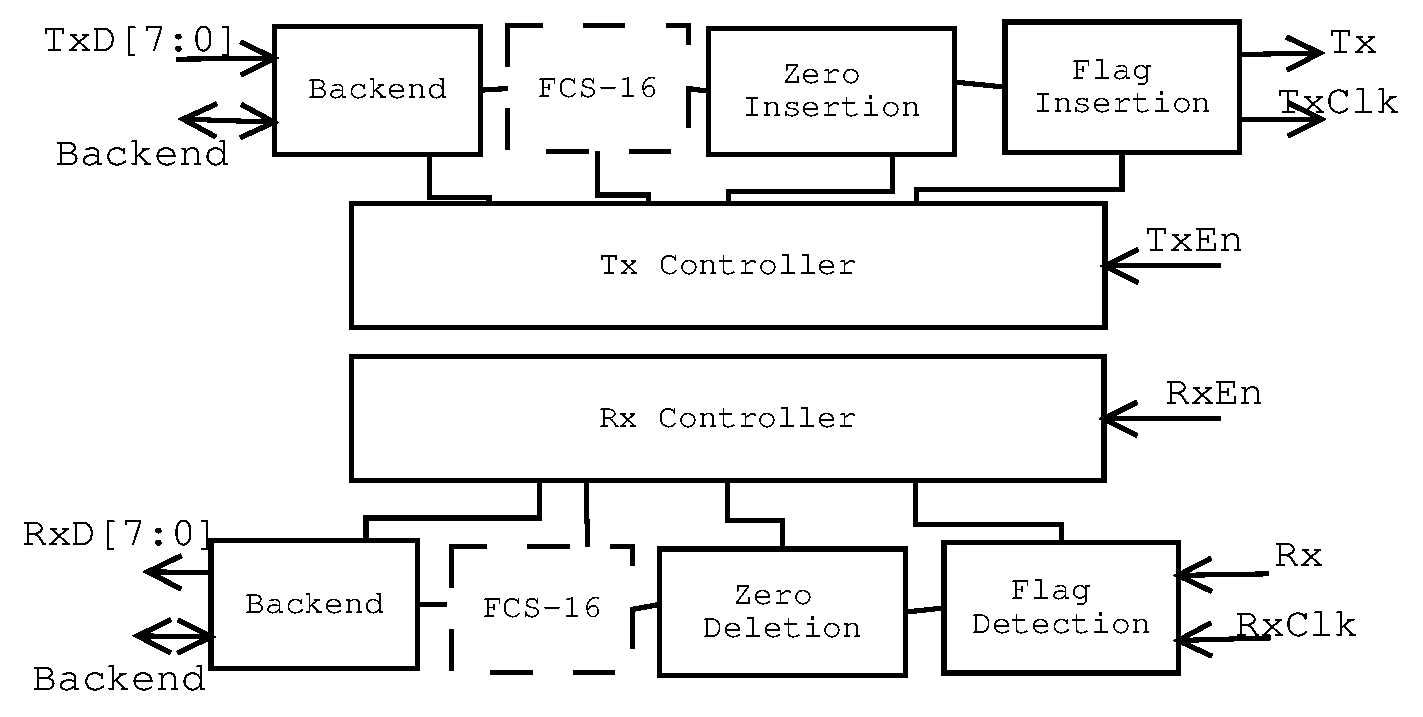
\includegraphics[angle=0,width=\textwidth]{HDLC_top.ps}
\caption{HDLC core}\label{Core}
\end{figure}

\begin{figure}[!h]
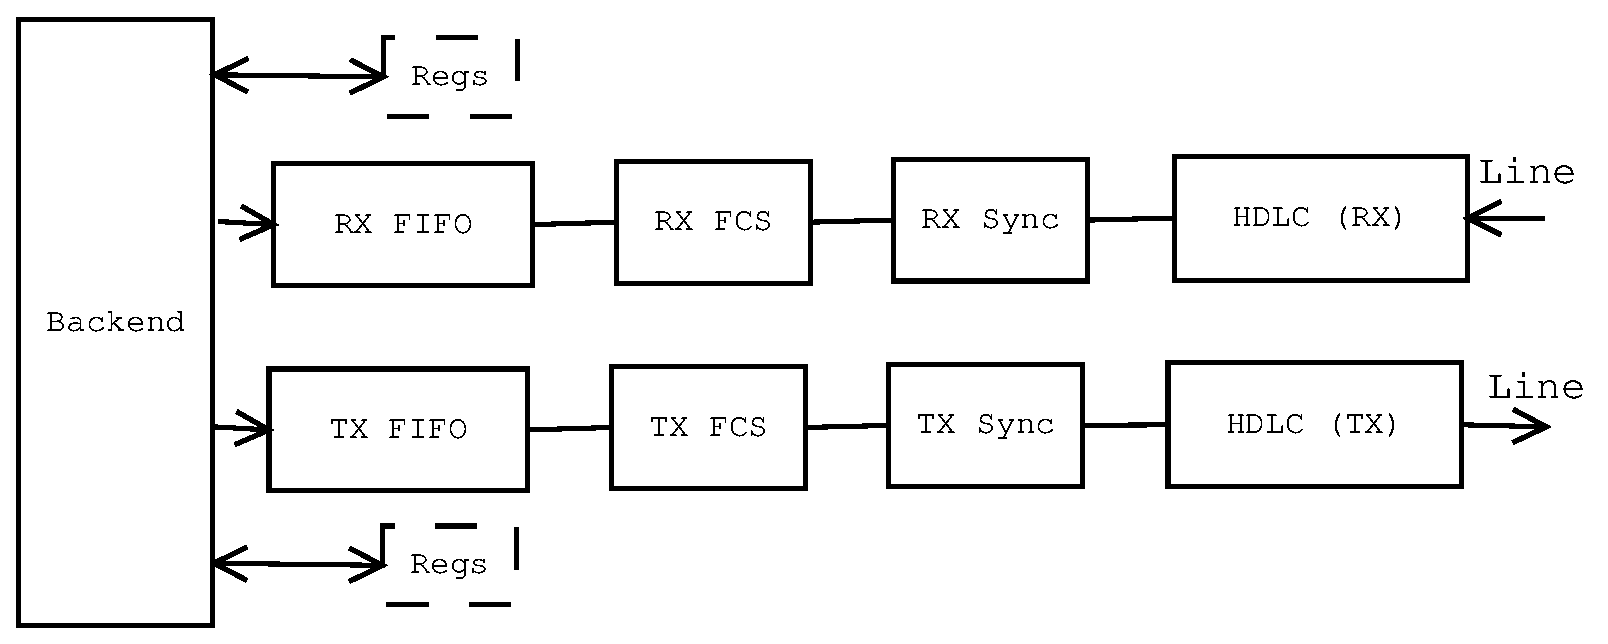
\includegraphics[angle=0,width=\textwidth]{HDLC_cont.ps}
\caption{HDLC controller}\label{controller}
\end{figure}


%%- New section -%%
%%------------------------------------------%%
\section{Testing and verifications}


\begin{tabular}{|l|l|l|}
\hline
Requirement & Test method & Validation method \\
\hline
\hline
Interface timing & &\\
\hline
& & \\
\hline
\hline
Functionality & & \\
\hline
\end{tabular}
\subsection{Simulation and Test benches}

\subsection{Verification techniques and algorithms}

\subsection{Test plans}

%%- New section -%%
%%------------------------------------------%%
\section{Implementations}
The  design is implemented using the VHDL language. The design is divided into three main blocks, serial Receive channel, Serial Transmit channel and the Top blocks.
The Receive and Transmit serial channels perform the HDLC
functionality. The Top blocks perform the FCS calculation (Which is
either  FCS-16 or FCS-32), the frame buffering the interface with the
back end system and the synchronization between the clocks. The FCS and Buffering can be changed by replacing the corresponding files.

\subsection{Scripts, files and any other information}
\begin{tabular}{|l|l|}
\hline
RX & \\
\hline
RxChannel.vhd & Top Rx Channel \\
Rxcont.vhd & Rx Controller \\
Zero\_detect.vhd & Zero detect and serial to parallel \\
flag\_detect.vhd & Flag detection \\
\hline
TX & \\
\hline
TxChannel.vhd & Top Tx channel \\
TXcont.vhd & Tx Controller\\
zero\_ins.vhd  & Zero insertion and parallel to serial \\
flag\_ins.vhd & Flag insertion \\
\hline
Top & \\
\hline
TxBuff.vhd&  Tx buffer\\
TxFCS.vhd &  Tx FCS-16\\
TxSync.vhd & Tx synchronization\\
RxBuff.vhd&  Rx buffer\\
RxFCS.vhd &  Rx FCS-16\\
RxSync.vhd & Rx synchronization\\
WB\_IF.vhd & WishBone interface\\
hdlc.vhd  & Top HDLC controller\\
\hline
\end{tabular}




\subsection{Design conventions and coding styles}

%%- New section -%%
%%------------------------------------------%%
\section{Reviews and comments}

%%- New section -%%
%%------------------------------------------%%
\section{References}


\end{document}
